Nesta seção, apresentamos os resultados da análise espectral do sinal, focando na comparação de diferentes filtros aplicados tanto a sinais de áudio quanto a imagens para remoção de ruído.

\subsection{Resultados da filtragem em sinal de áudio}
As figuras ~\ref{fig:audio_butterworth_spectrums} e ~\ref{fig:audio_elliptical_spectrums} mostram os espectros de frequências e as respostas em frequência dos filtros Butterworth e Elíptico em um áudio ruidoso.

\begin{figure}[H]
    \centering
    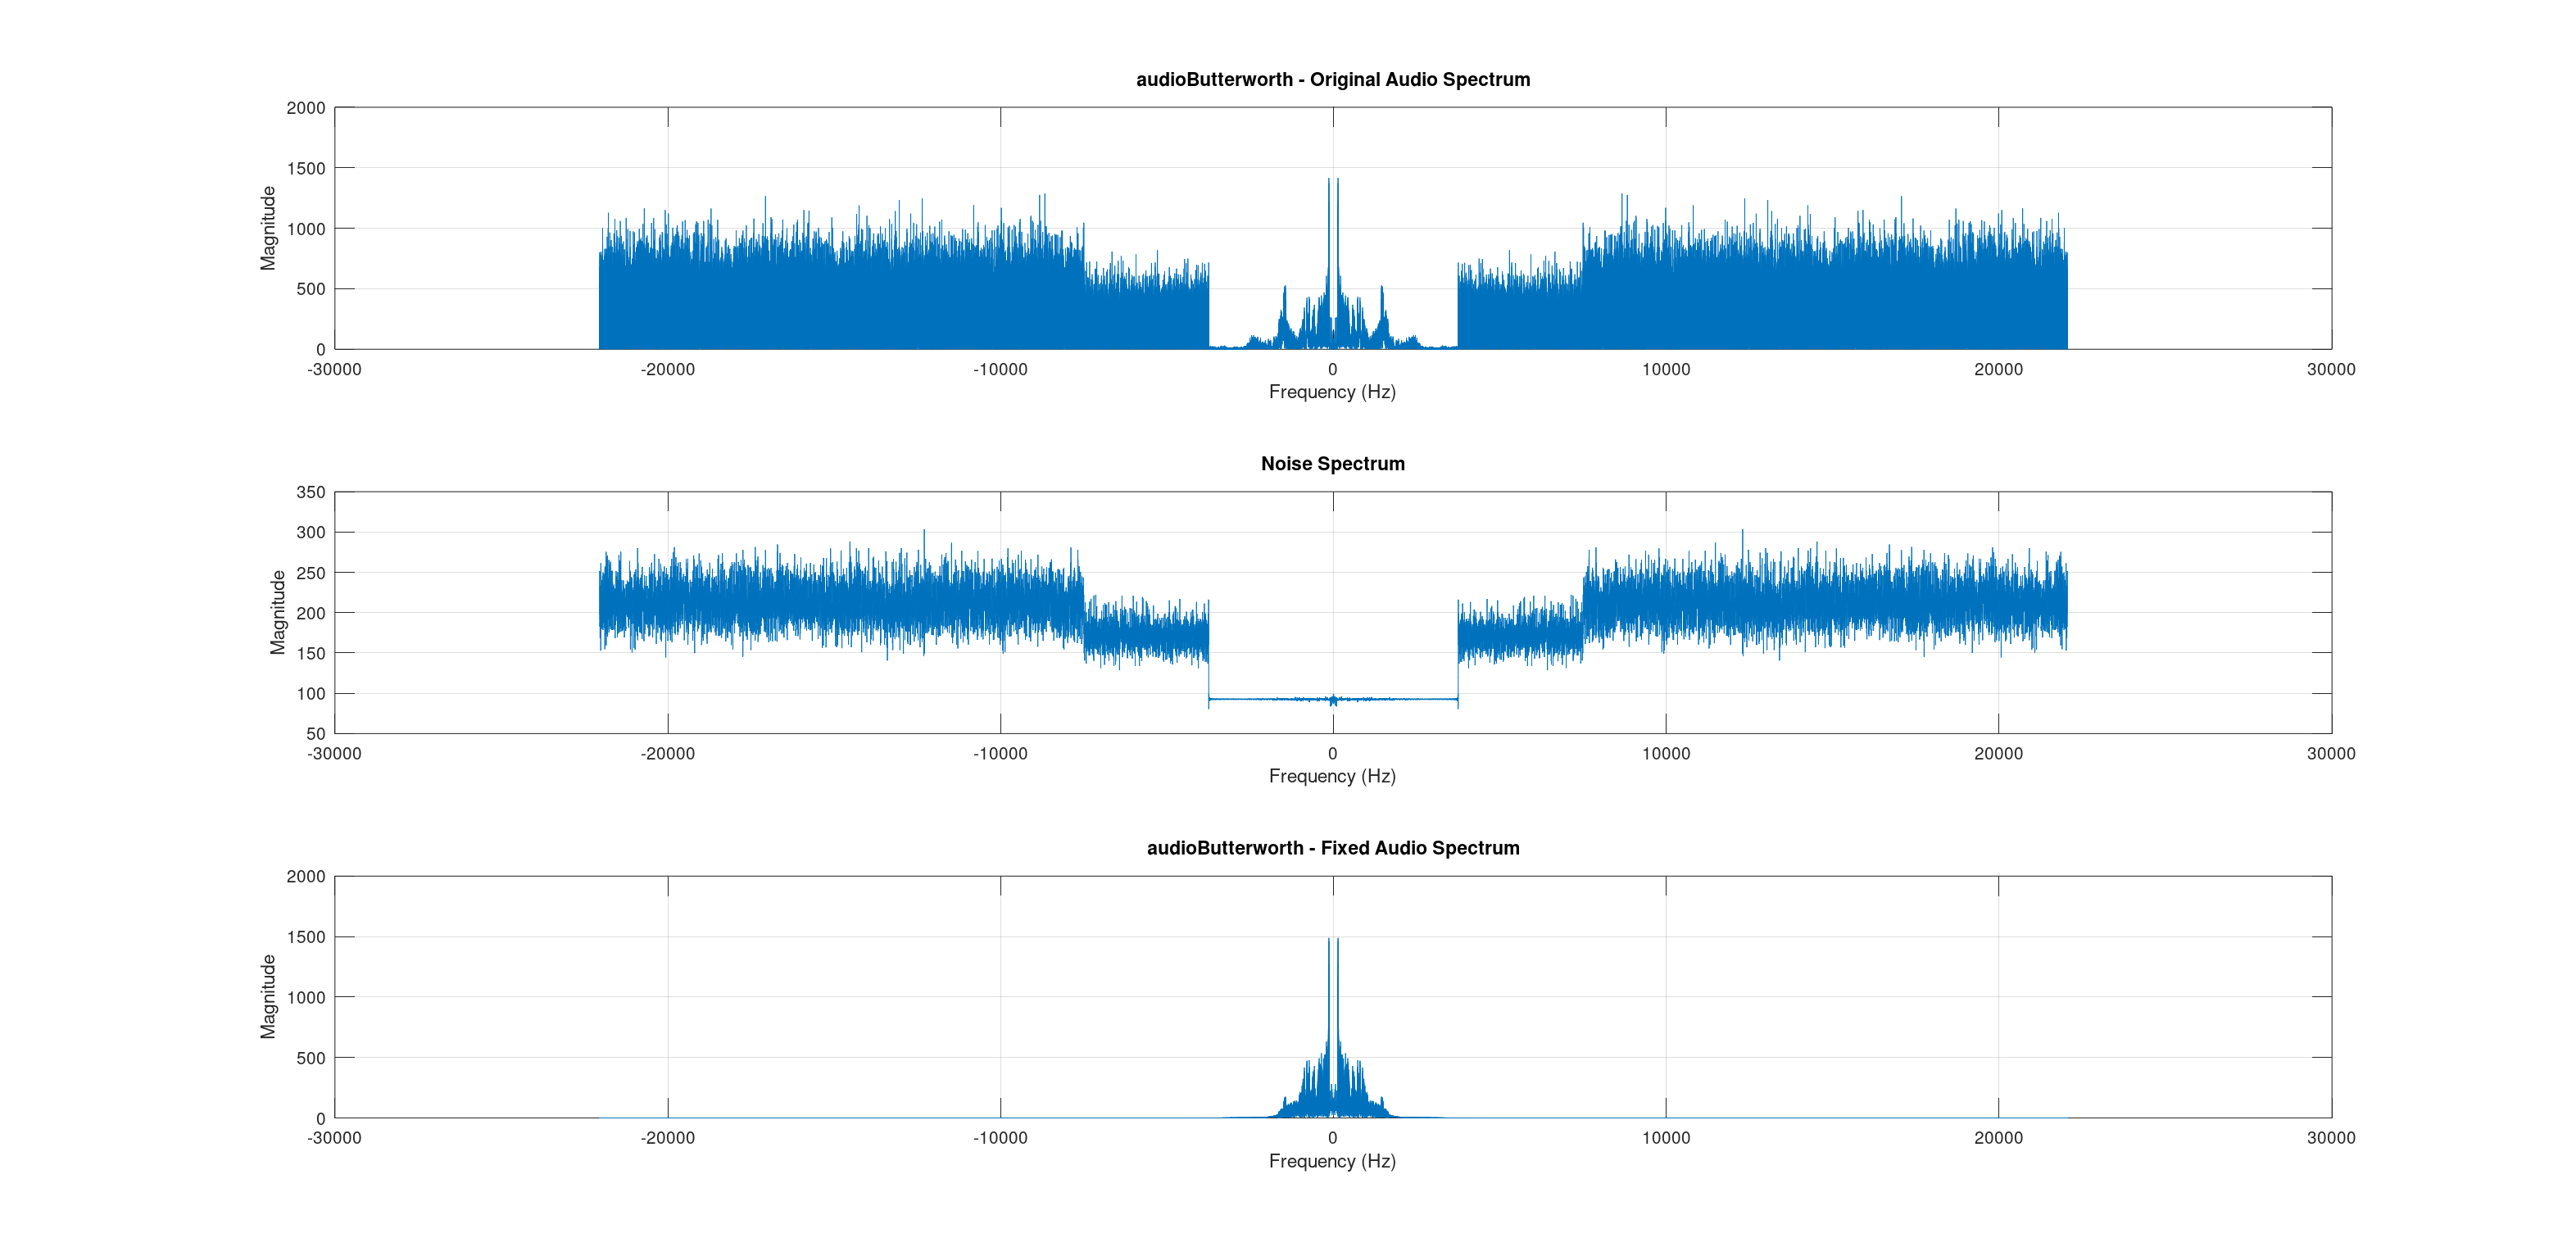
\includegraphics[width=1\linewidth]{03_results/assets/audio_butterworth_spectrums.png}
    \caption{Espectro de frequência do sinal de áudio antes e após a aplicação do filtro Butterworth.}
    \label{fig:audio_butterworth_spectrums}
\end{figure}

O filtro \textbf{Butterworth} é caracterizado por sua resposta suave e sem ondulação, proporcionando uma atenuação gradual das frequências fora da faixa desejada. Este tipo de filtro é muito útil para preservar a integridade do sinal enquanto remove ruídos de alta frequência. Na figura \ref{fig:audio_butterworth_spectrums}, podemos observar como o filtro atua suavemente, permitindo que a faixa passante do sinal de áudio se mantenha praticamente intacta, enquanto o ruído de alta frequência é atenuado.

\begin{figure}[H]
    \centering
    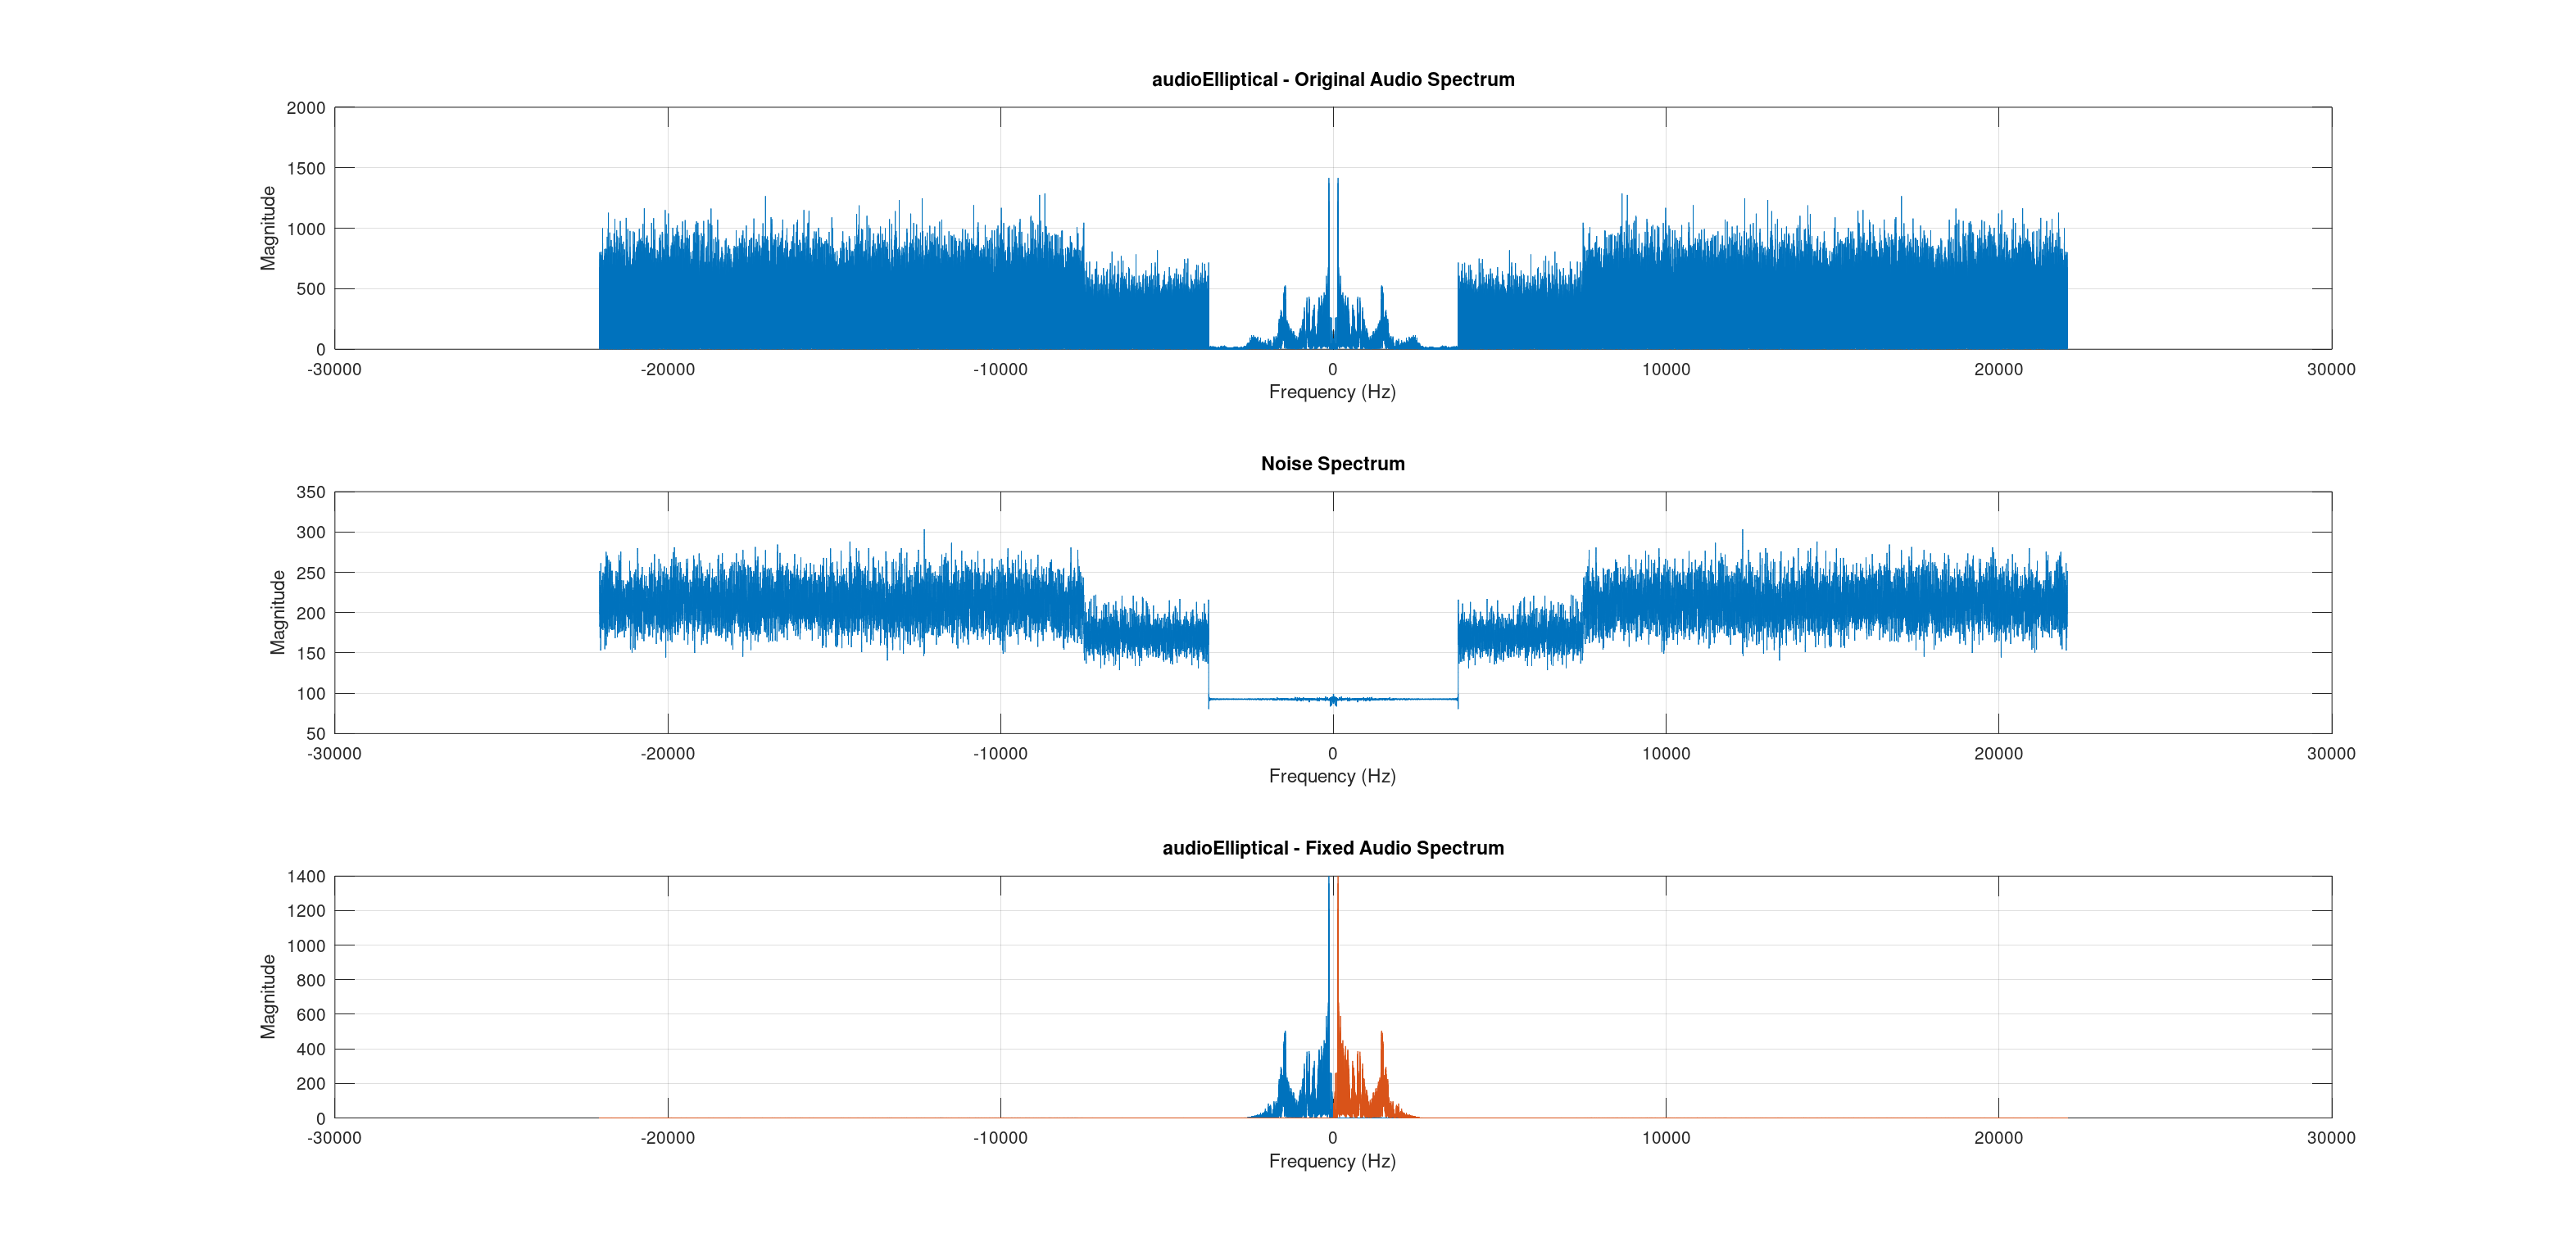
\includegraphics[width=1\linewidth]{03_results/assets/audio_elliptical_spectrums.png}
    \caption{Espectro de frequência do sinal de áudio antes e após a aplicação do filtro Elíptico.}
    \label{fig:audio_elliptical_spectrums}
\end{figure}

O filtro \textbf{Elíptico}, diferente do Butterworth, apresenta uma atenuação mais agressiva nas frequências fora da faixa passante. A principal característica desse filtro é a \textbf{ondulação} na resposta de magnitude, tanto na faixa passante quanto na faixa de rejeição. Isso permite uma filtragem mais eficiente, removendo frequências indesejadas de forma mais agressiva. No entanto, as oscilações na transição entre a faixa passante e a faixa de rejeição podem resultar em distorções perceptíveis, especialmente quando a integridade do sinal precisa ser preservada.

\subsection{Resultados da filtragem em Imagem Digital}
Como apresentado na Figura ~\ref{fig:image_original_plus_noise}, foi carregada uma imagem original 256x256 pixels, e aplicado um ruído senoidal na mesma.

\begin{figure}[H]
    \centering
    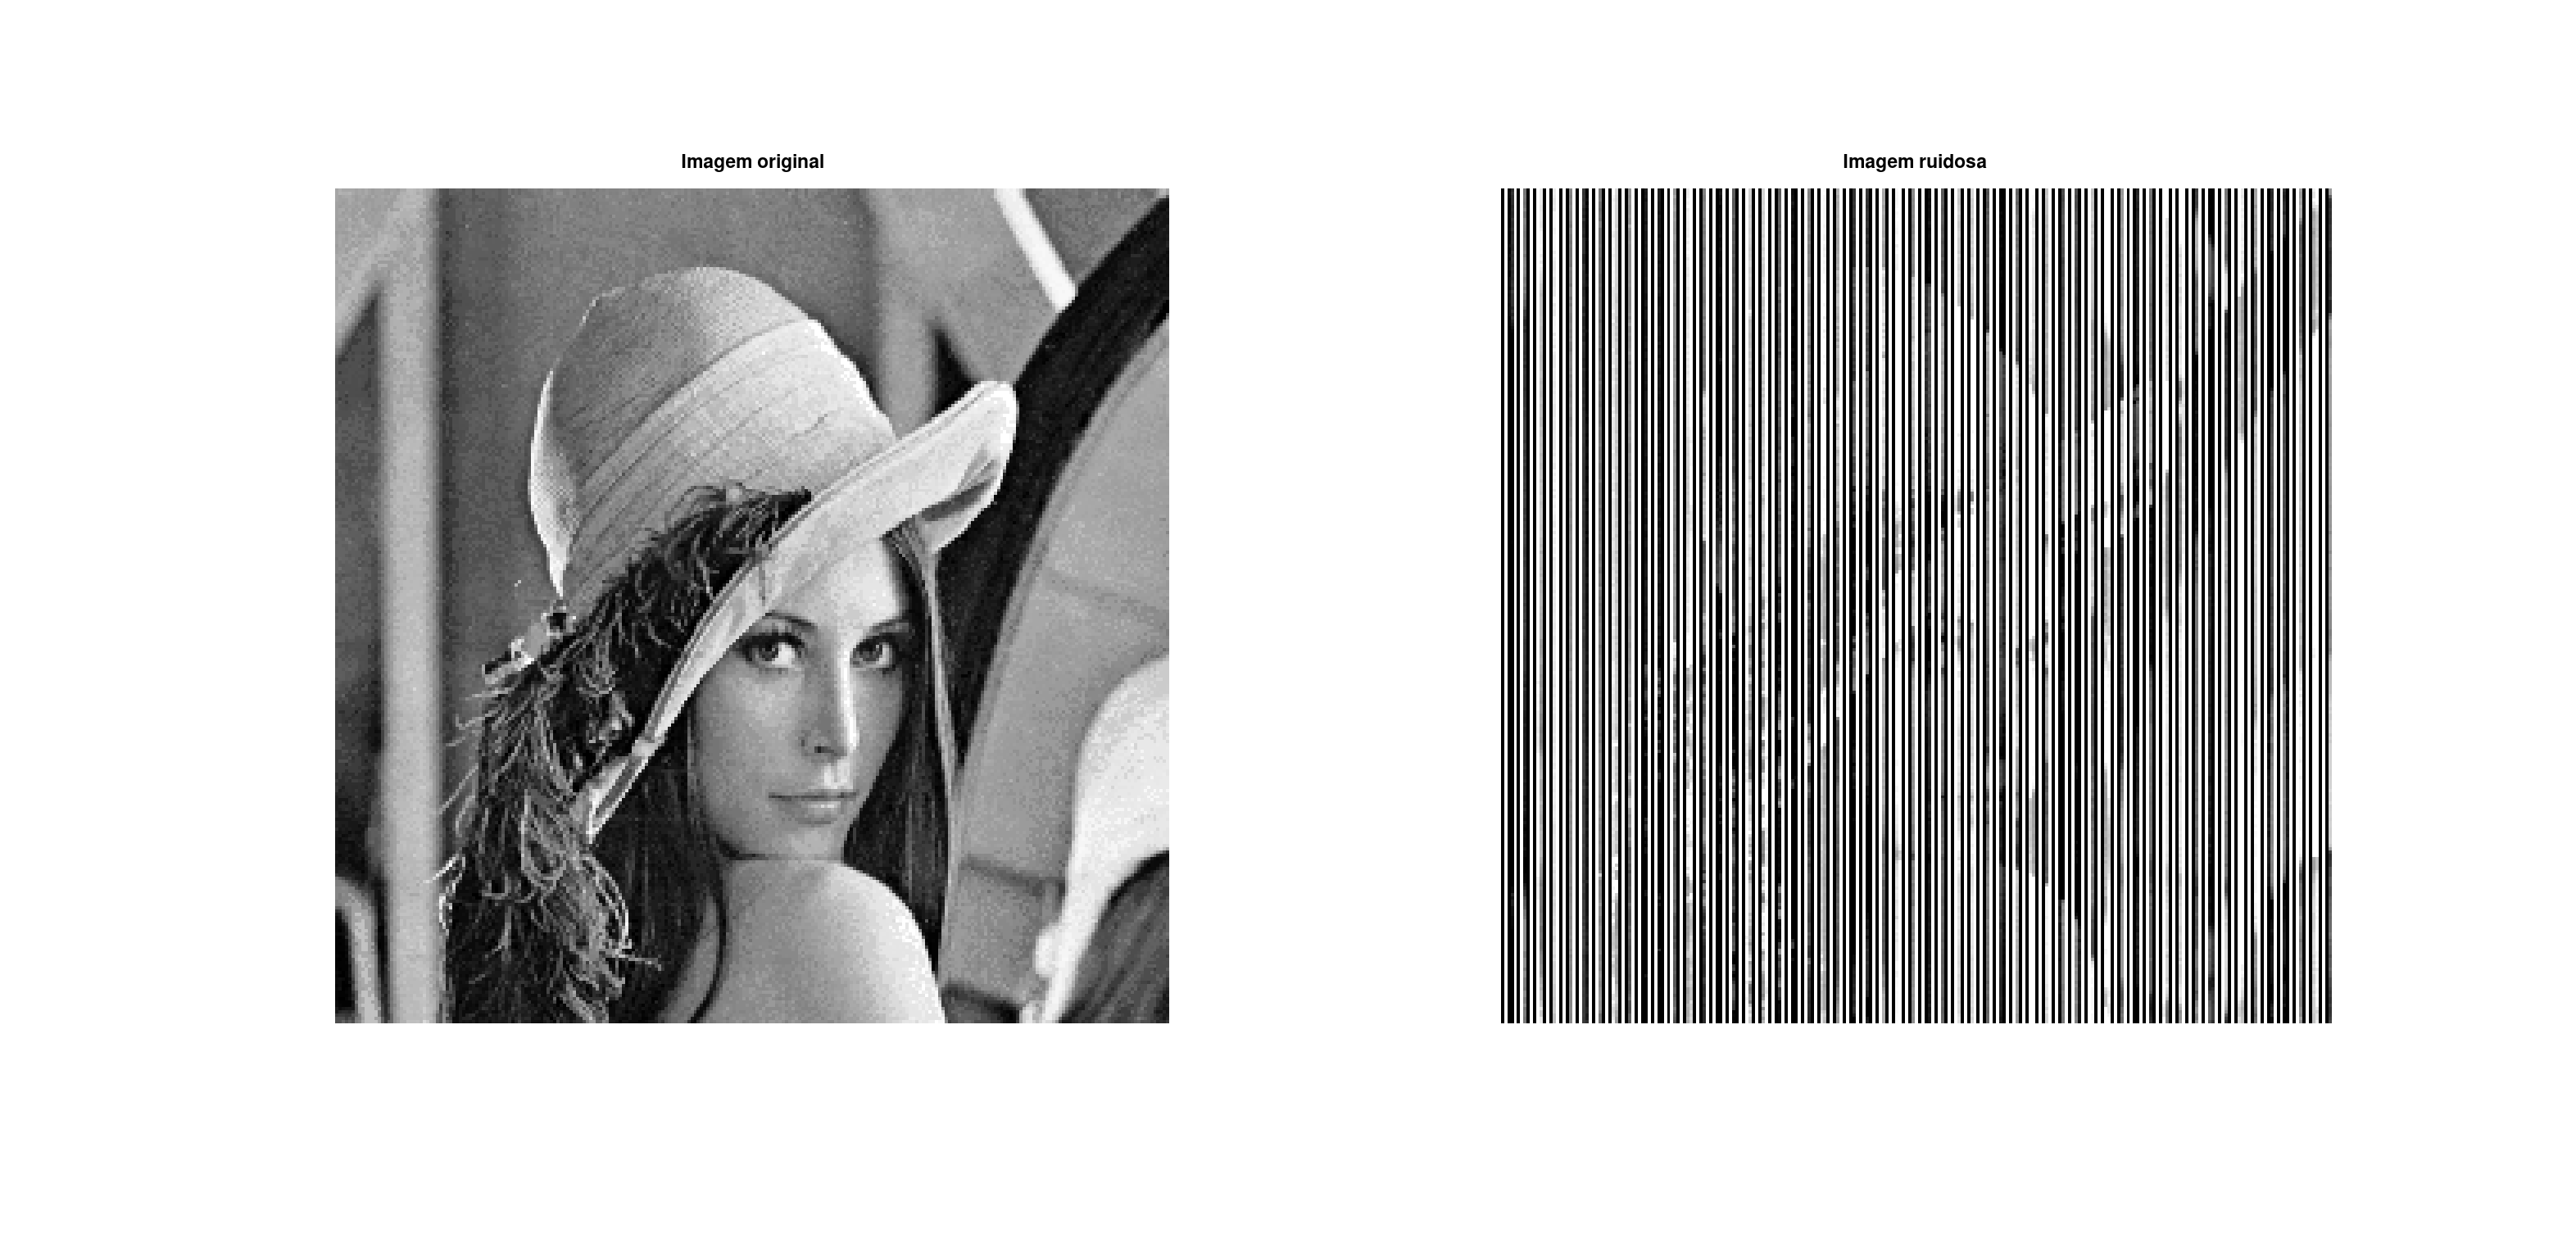
\includegraphics[width=1\linewidth]{03_results/assets/image_original_plus_noise.png}
    \caption{Imagem original e imagem ruidosa}
    \label{fig:image_original_plus_noise}
\end{figure}

A figura \ref{fig:image_direct_remove_noise} mostra o efeito de uma \textbf{remoção direta de ruído} na imagem. Embora simples, essa técnica pode resultar em perda de detalhes finos e pode afetar as bordas ou áreas de transição entre regiões de diferentes intensidades. Em imagens com ruído de alta frequência, o método direto pode ser útil, mas suas limitações incluem a possível suavização excessiva de áreas importantes da imagem.

\begin{figure}[H]
    \centering
    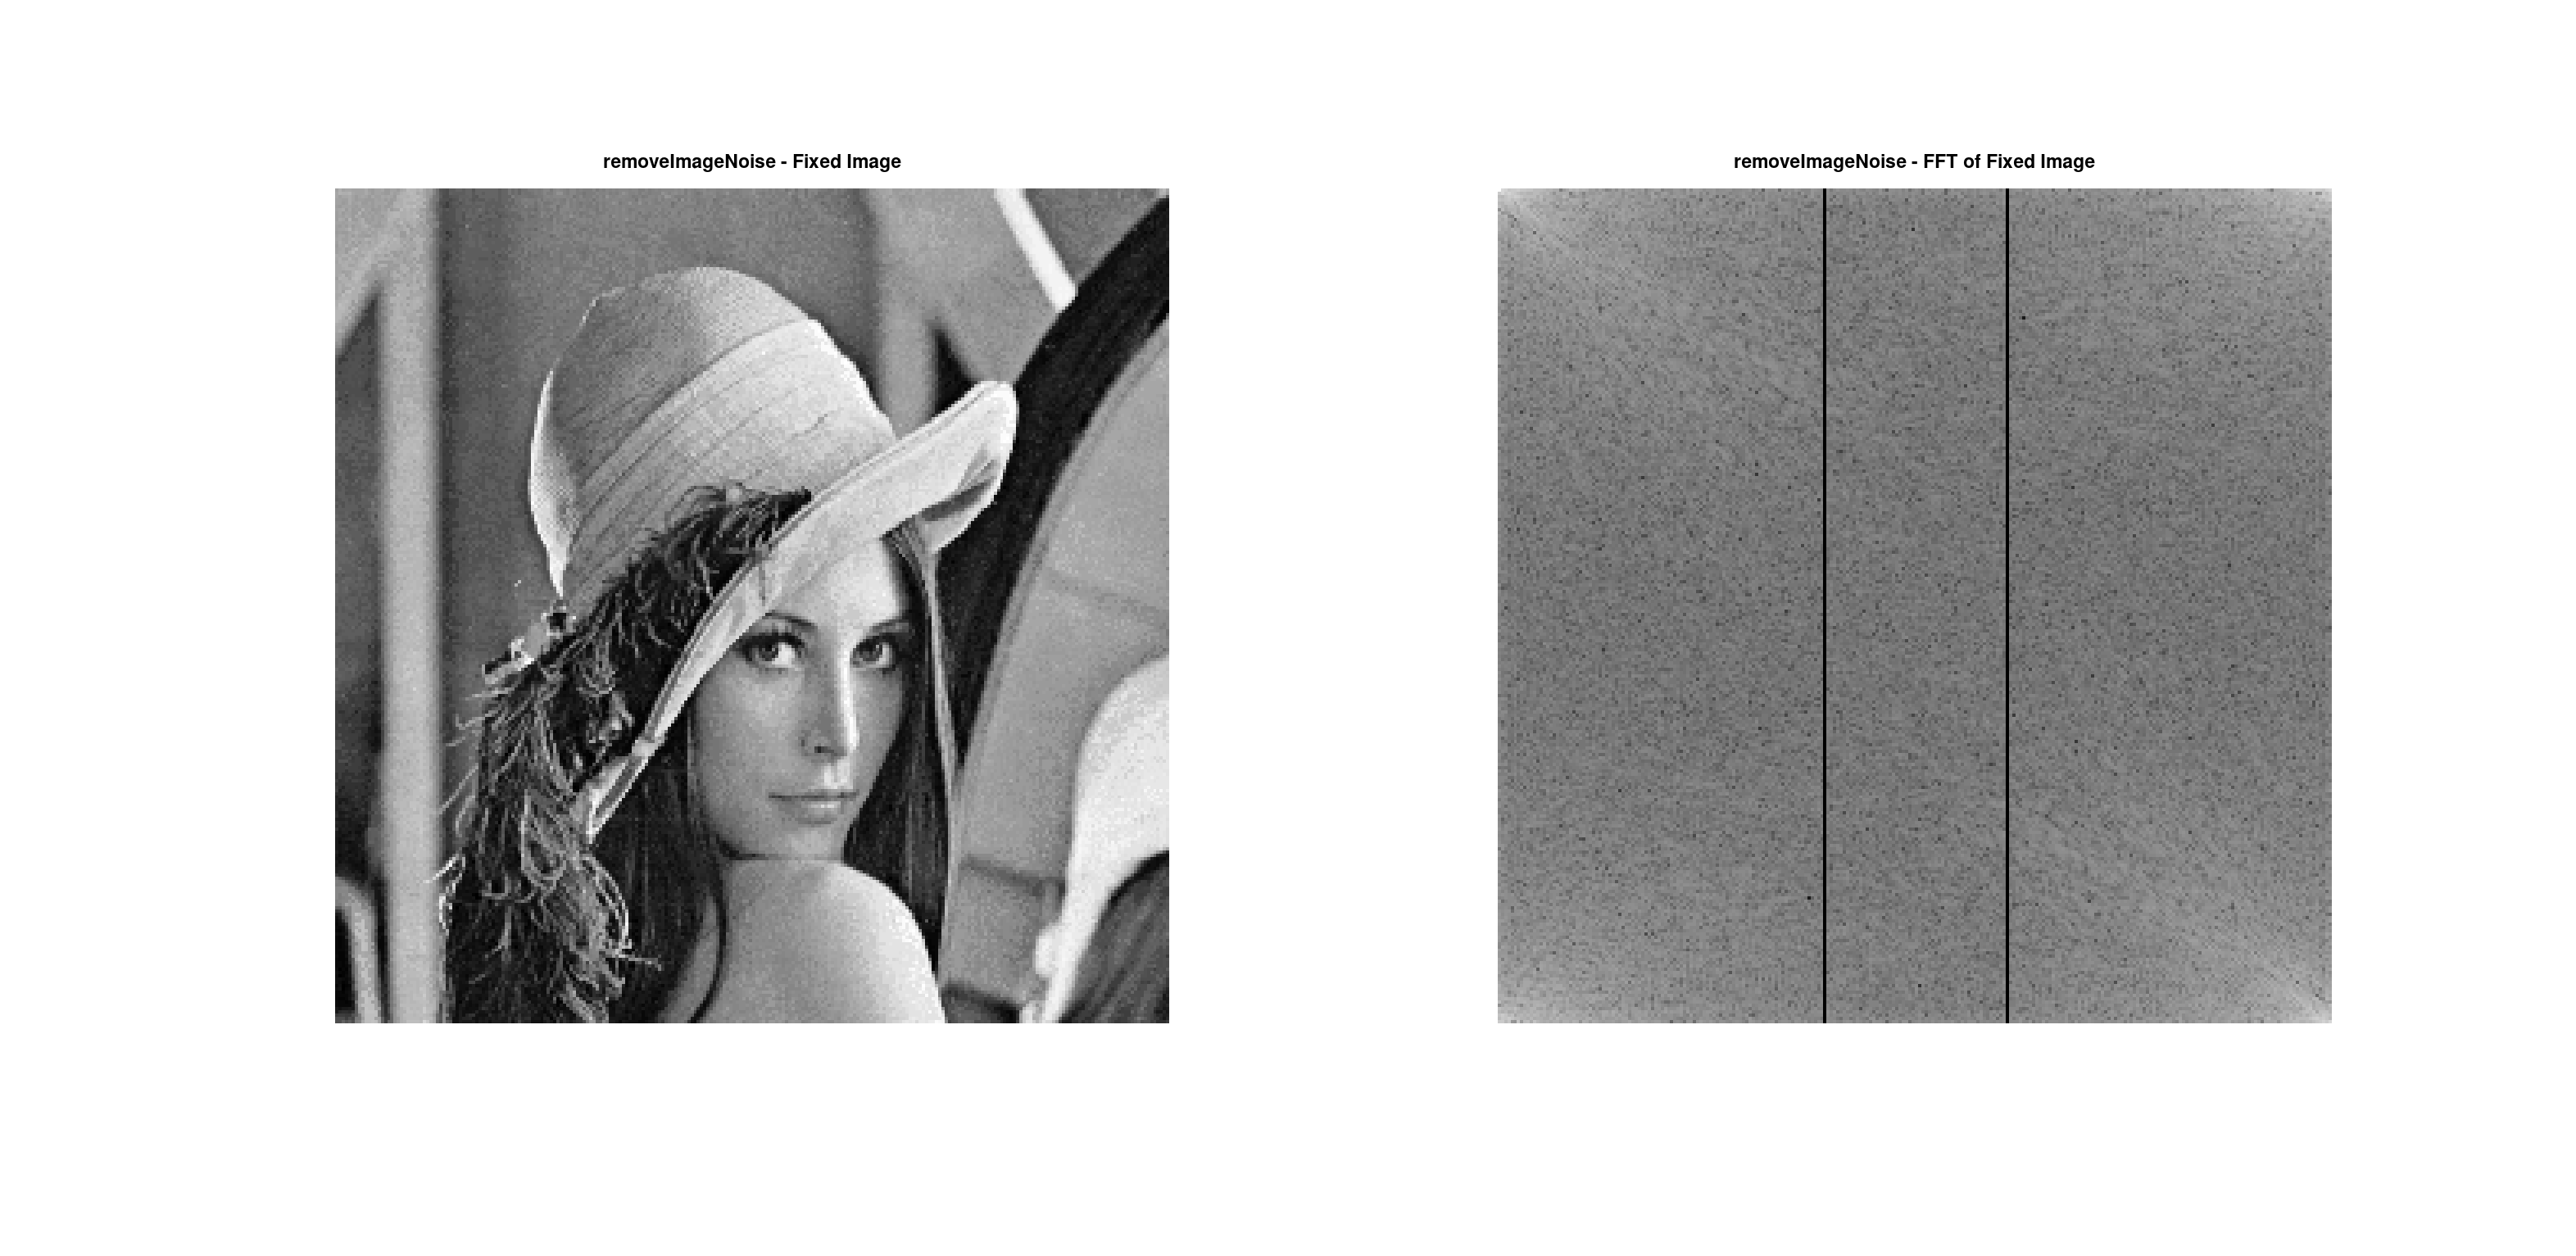
\includegraphics[width=1\linewidth]{03_results/assets/image_direct_remove_noise.png}
    \caption{Imagem filtrada e seu espectro com a remoção direta do ruído.}
    \label{fig:image_direct_remove_noise}
\end{figure}

Na figura \ref{fig:image_butterworth}, vemos a imagem original ao lado da imagem filtrada com o filtro Butterworth. Este filtro é eficaz na remoção de ruído de alta frequência sem afetar significativamente as bordas ou detalhes importantes da imagem. Ele suaviza as transições, mas mantém a maior parte da estrutura da imagem. Como resultado, o filtro Butterworth é uma escolha adequada quando se deseja minimizar o impacto visual nas imagens filtradas, especialmente em áreas que contêm detalhes importantes.

\begin{figure}[H]
    \centering
    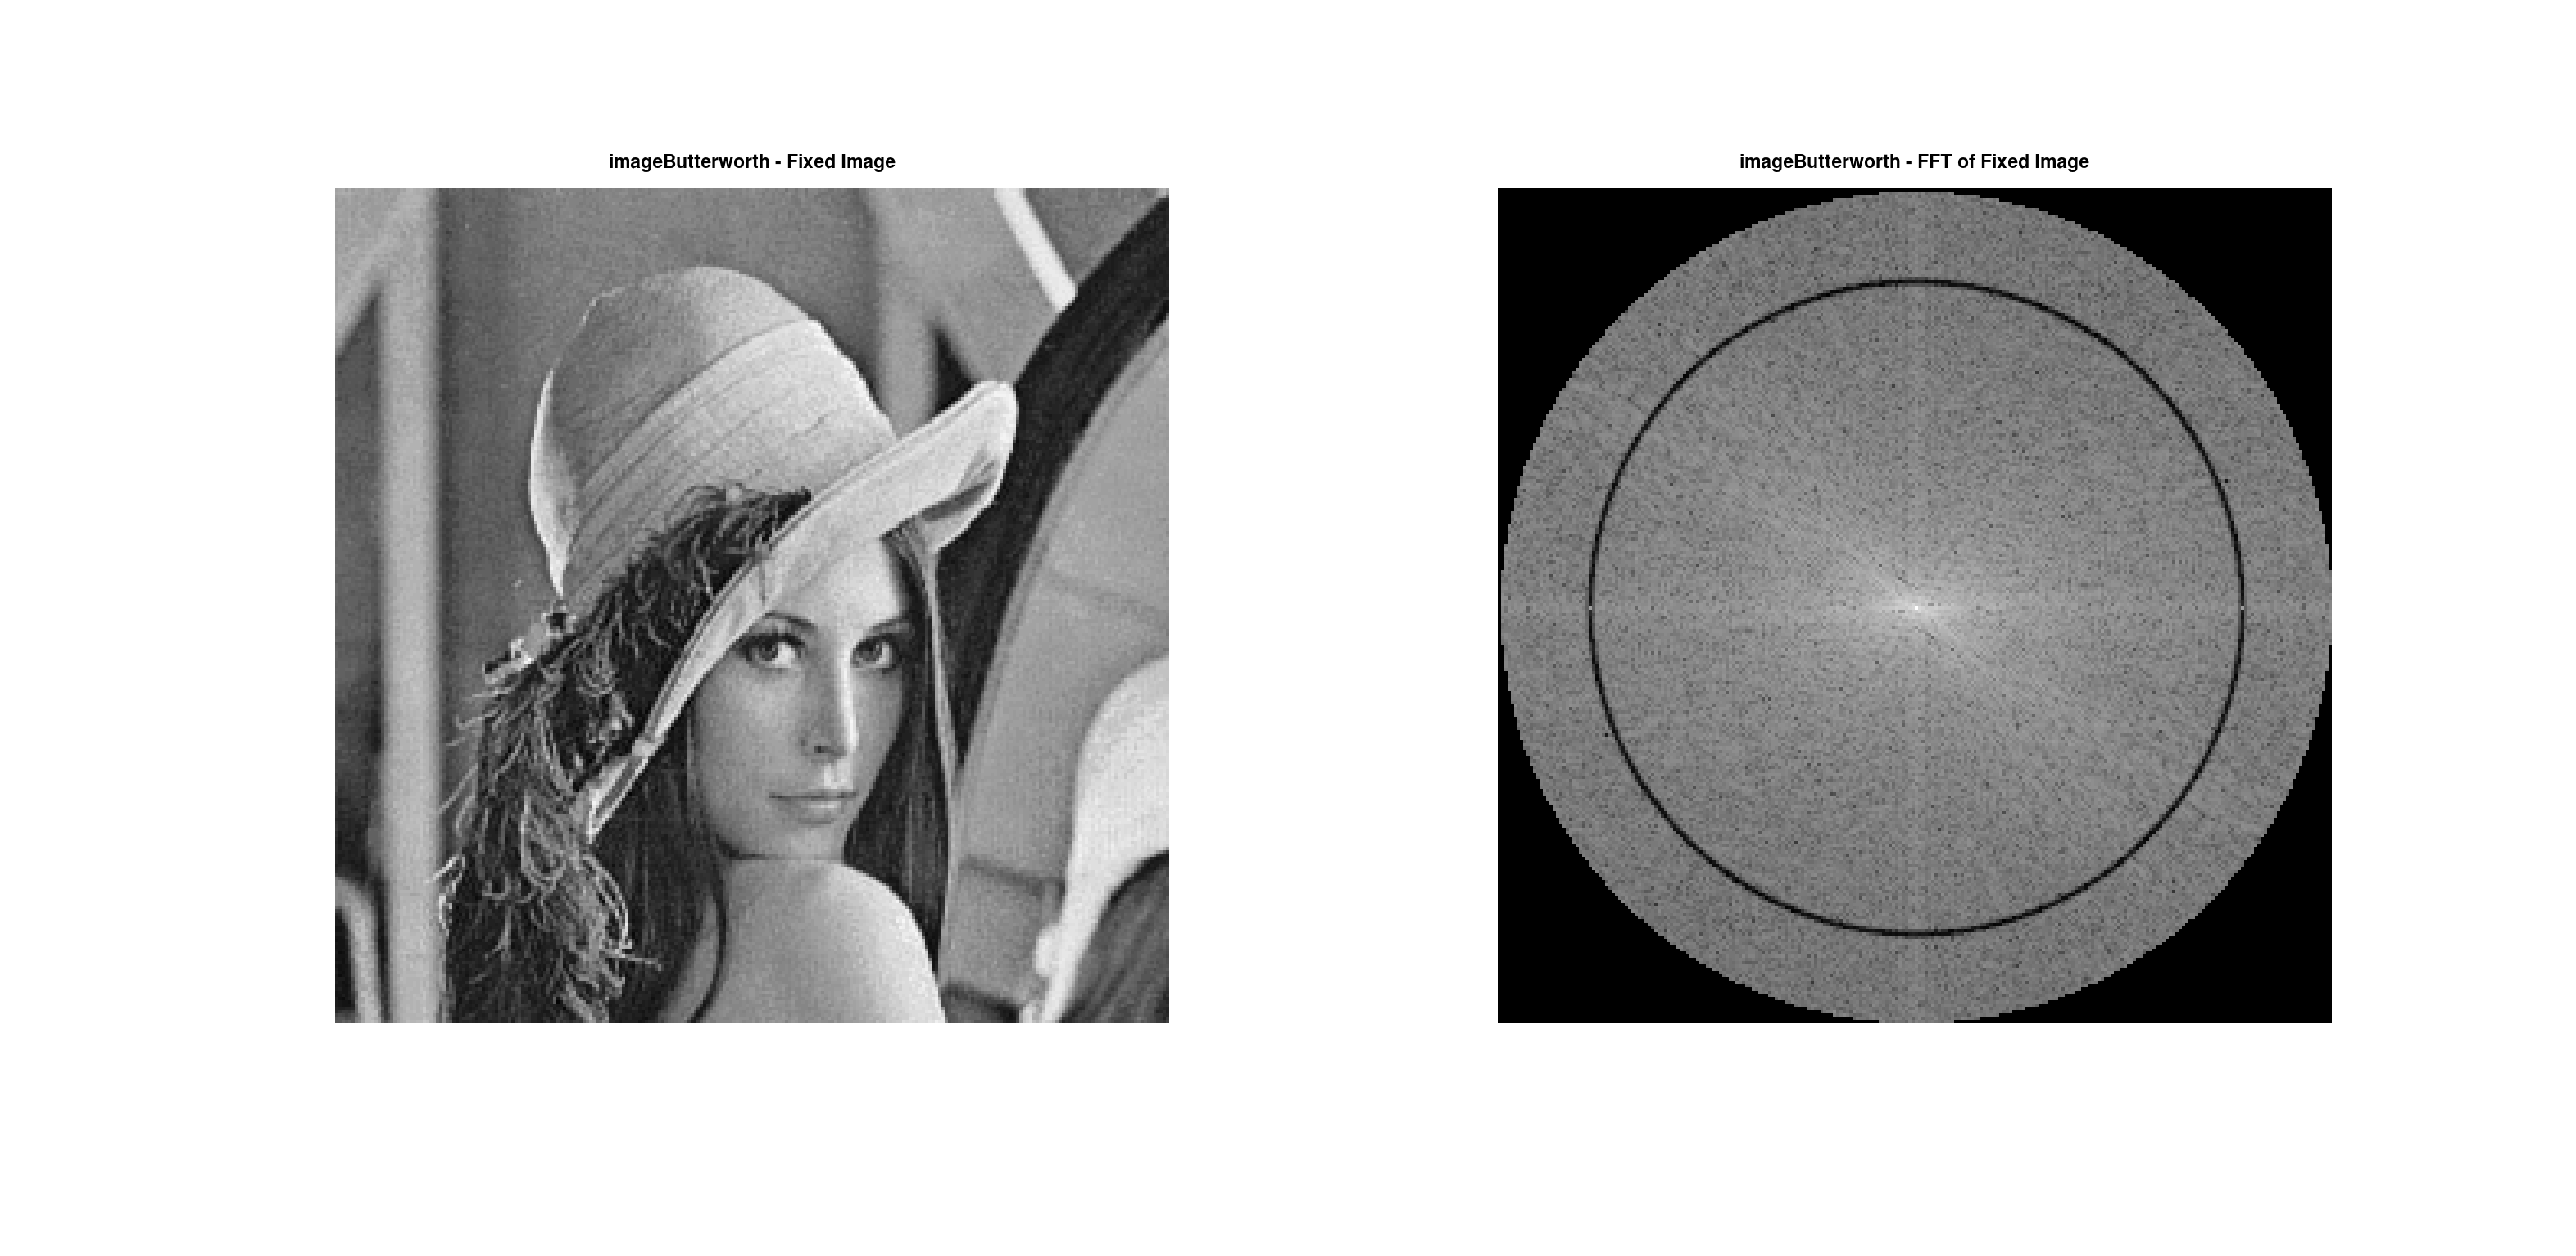
\includegraphics[width=1\linewidth]{03_results/assets/image_butterworth.png}
    \caption{Imagem filtrada e seu espectro com o filtro Butterworth.}
    \label{fig:image_butterworth}
\end{figure}

A figura \ref{fig:image_chebyshev} mostra a aplicação do filtro \textbf{Chebyshev}. Este filtro, sendo mais agressivo do que o Butterworth, apresenta uma resposta em frequência mais acentuada, permitindo uma remoção mais eficaz de ruídos em frequências específicas. No entanto, ele também pode introduzir distorções visíveis, especialmente em áreas com transições suaves, como as bordas da imagem. As oscilações na resposta de frequência podem resultar em artefatos indesejáveis, tornando-o uma escolha mais arriscada quando a preservação da qualidade visual é crítica.

\begin{figure}[H]
    \centering
    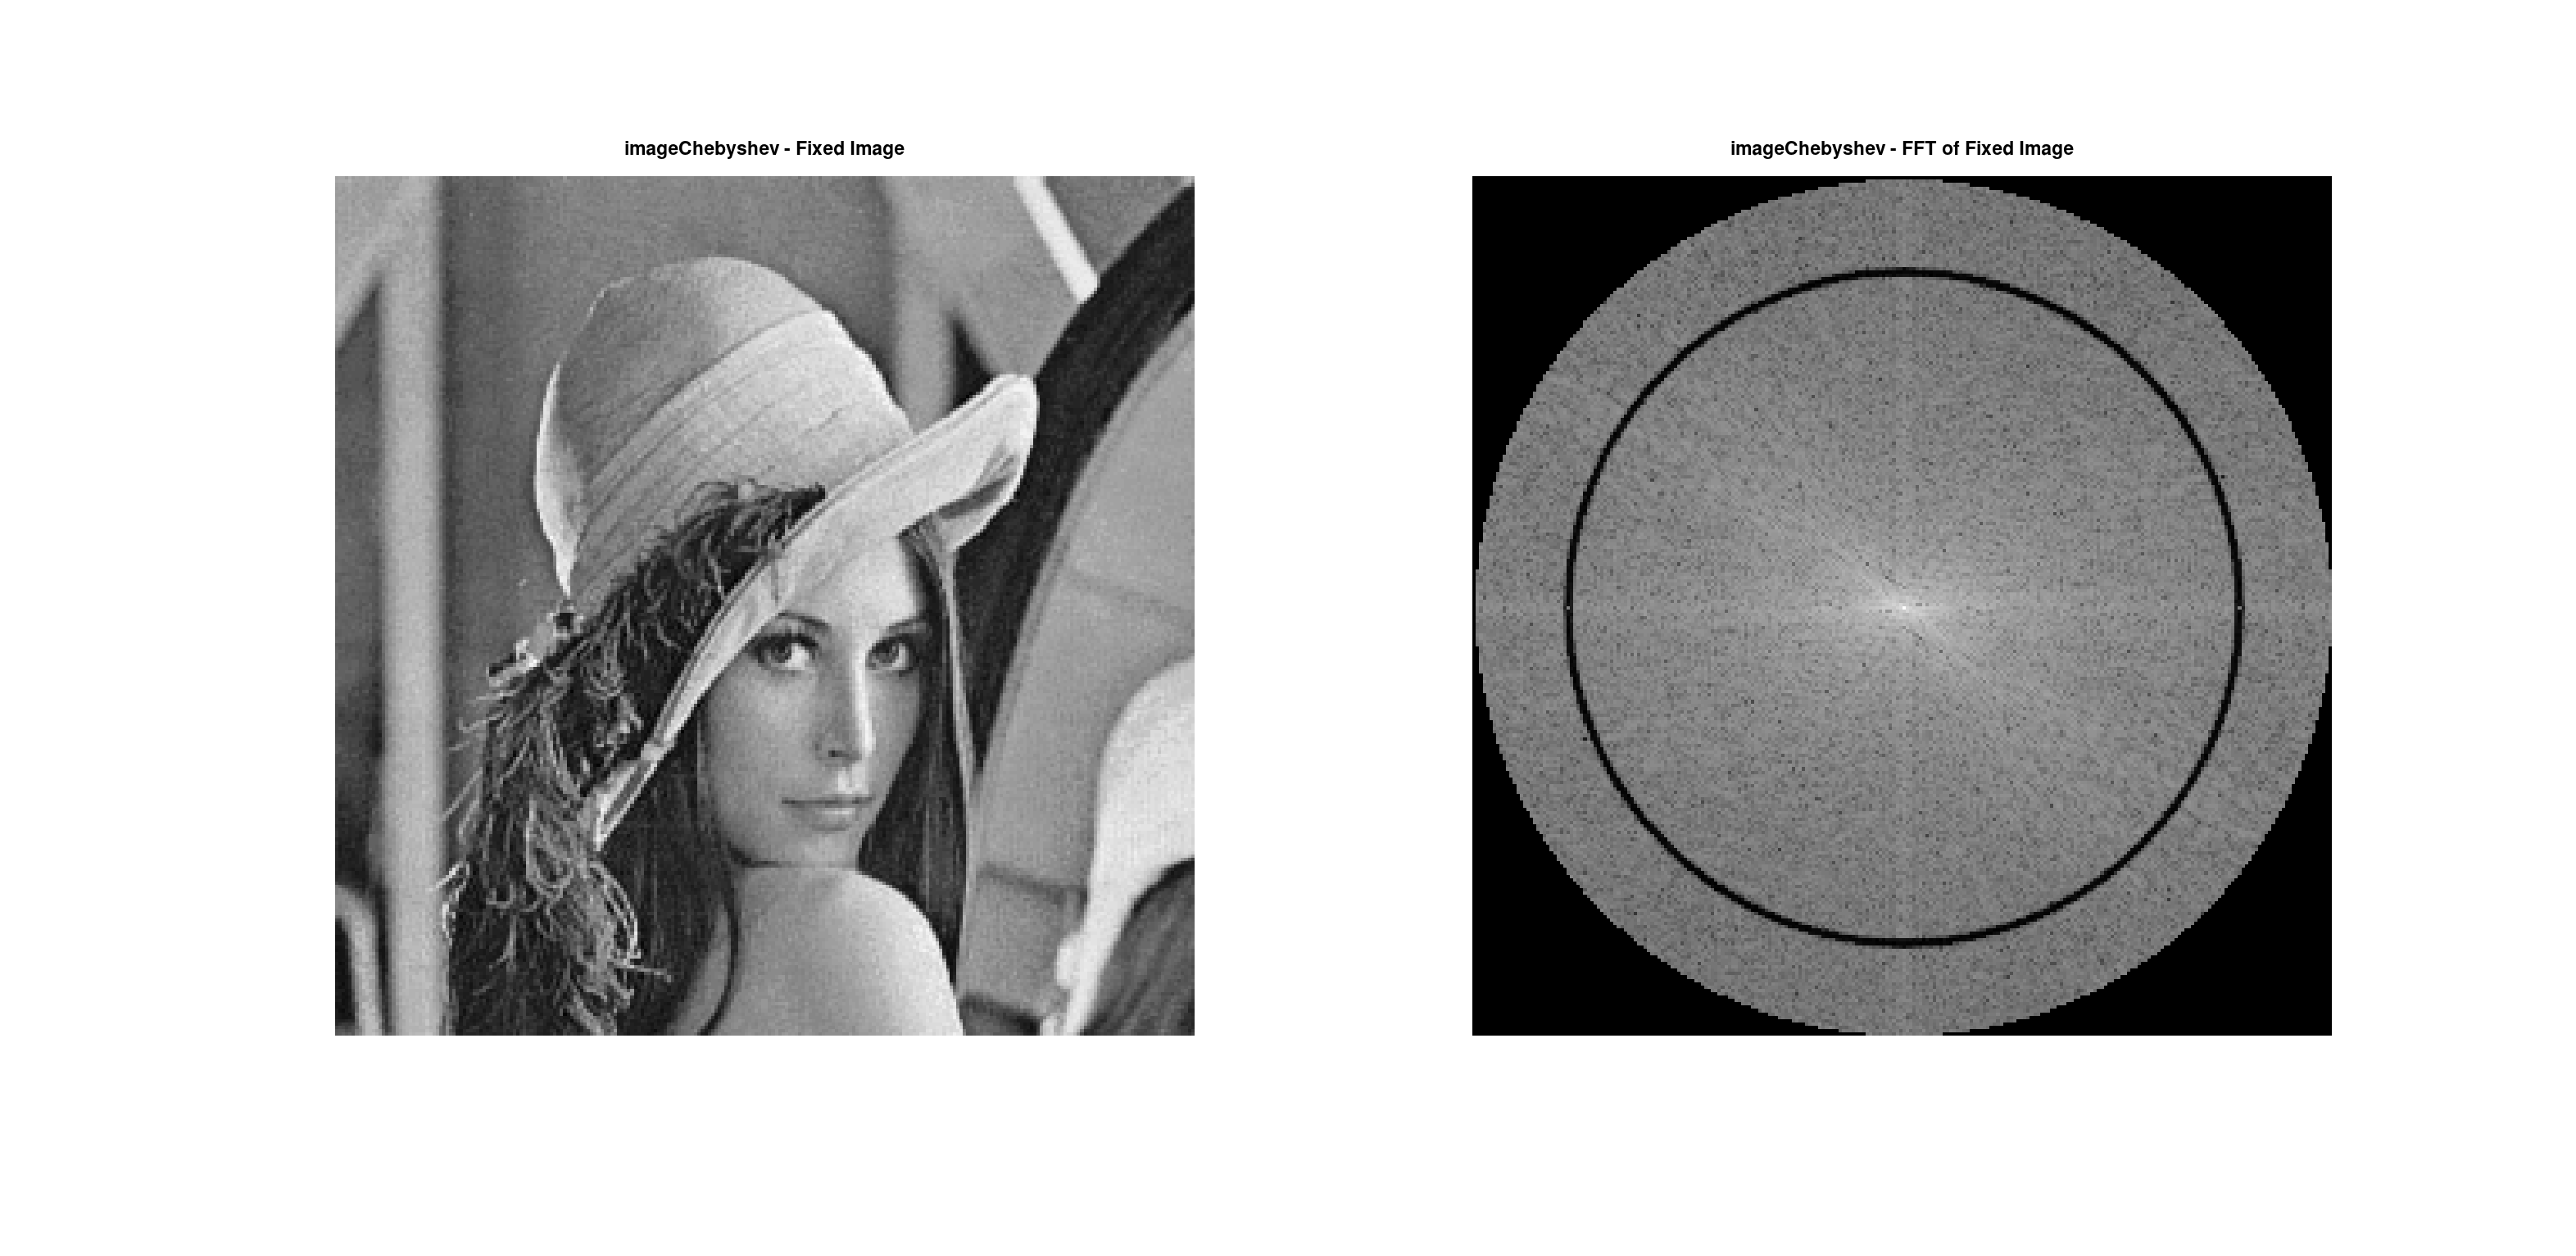
\includegraphics[width=1\linewidth]{03_results/assets/image_chebyshev.png}
    \caption{Imagem filtrada e seu espectro com o filtro Chebyshev.}
    \label{fig:image_chebyshev}
\end{figure}
